\DiaryEntry{Convex Optimization, 1}{2015-12-07}{Optimization}

\subsection{Convex Sets}

Consider two points $P\_1, P\_2$ in an n-dimensional space $\mathcal{R}^n$. A line $l(\theta)$ connecting these two points is given by

\[
l(\theta) = \theta P_1 + (1-\theta) P_2, \quad \theta \in [0,1]
\]

If $\theta=1$, we are at $P_1$, for $\theta=0$, we are at $P_2$. For all values of $\theta$ in $[0,1]$, we are somewhere in between the two points.

A set $\mathcal{C}$ is called convex, if for any two points $P_1, P_2
\in \mathcal{C}$, the line connecting these two points is also in $\mathcal{C}$; i.e. $l(\theta) \in \mathcal{C}$ for $\theta$ in $[0,1]$.

\subsubsection{Hyperplanes}

A hyperplane is given by the set

\[ \{ x | a^T (x - x_0) = 0 \} \]

where $x, a, x_0$ are all n-dimensional vectors; $x_0$ being the displacement of the hyperplane from the origin and $a$ denoting the normal vector of the plane.

\paragraph{Two-dimensional Example}

In this case $x = (x , y)^T$, $a = (a_1 , a_2)^T$, $x_0 = (x_0 , y_0)^T$ and we have

\[
a_1(x - x_0) + a_2(y - y_0) = 0 \rightarrow y = \frac{a_1 x_0 + a_2 y_0}{a_2} - \frac{a_1}{a_2}x
\]

If $a = (1 , 1)^T$ and $x_0 = (1 , 0)^T$, we have $y = 1-x$.

\subsubsection{Halfspaces}

A halfspace is the area ``below'' a hyperplane; i.e.~the set

\[ \{ x | a^T (x - x_0) \leq 0 \} \]

\begin{figure}[H]
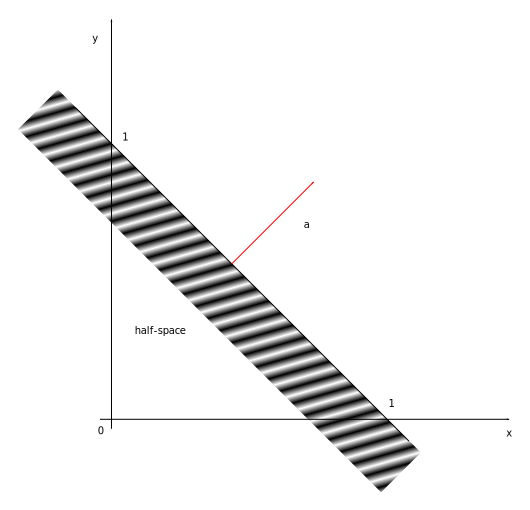
\includegraphics[scale=0.7]{images/convex_opt_01.png}
\end{figure}

A halfspace is always a convex set.

\subsubsection{Polyhedra}

Polyhedras $\mathcal{P}$ are combinations of halfspaces; i.e.

\[
\mathcal{P} = \{ x | A x \leq b, Cx = d  \}
\]

$A, C$ are matrices, $b, d$ are vectors.

\subsection{Convex Functions}

A convex function $f(x)$ is characterised by

\[
f(\theta x + (1-\theta)y) \leq \theta f(x) + (1-\theta)f(y)
\]

We can interpret the LHS a inputing any point on the line between
$x, y$ into the function. Then the function must be below (or equal) the line connecting the points $x, f(x)$ and $y, f(y)$ (the RHS).

\begin{figure}[H]
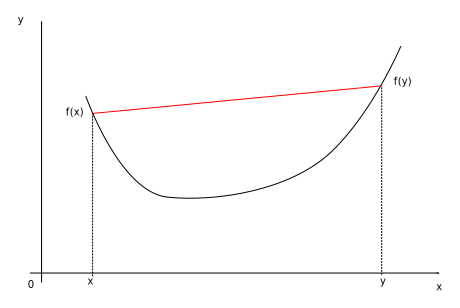
\includegraphics[scale=0.7]{images/convex_opt_02.png}
\end{figure}

An equivalent condition is

\[
f(y) \geq f(x) + \nabla f(x)^T (y-x)
\]

where the RHS is the tangent to $f(x)$ at point $(x, f(x))$.

And another equivalent condition is that

\[
\nabla^2 f(x) \geq 0
\]

i.e.~the second derivative (matrix) is positive (semi-definite).

\subsubsection{Basic Convexity Conditions}

There are some basic rules about convex functions:

\begin{itemize}
\item
  Linear and affine functions are convex
\item
  Quadratic functions $f(x) = 1/2 x^T P x + q^T x + r$ are convex if $\nabla^2 f(x) = P $ is positive semidefinite.
\item
  The function $e^{a x}$ is convex
\item
  The function $|x|^p, p \geq 1$ is convex
\item
  The functions $\log(x)$ and $x \log(x)$ are convex
\item
  Every norm is convex: Every norm $|x|$ (in order to
  be a norm) fulfills the triangle inequality:
  $|x+y| \leq |x| + |y|$. This can be stated differently in that we write
\end{itemize}

\[
\|\theta x+(1-\theta) y\| \leq \|\theta x\| + \|(1-\theta) y\| = \theta \|x\| + (1-\theta) \|y\|
\]

Sublevel sets of convex functions are convex sets: An $\alpha-$sublevel $C_\alpha$ of a function is defined as $C_\alpha = \{ x | f(x) \leq \alpha \}$. Assume that $x,y \in C_\alpha$, then we have $f(x), f(y) \leq \alpha$. We have

\[
f(\theta x + (1-\theta)y) \leq \theta f(x) + (1-\theta) f(y) \leq \theta \alpha + (1-theta) \alpha = \alpha
\]

where the first inequality follows from convexity of $f$ and the second inequality follows because of $x,y \in C_\alpha$.

\subsubsection{Convexity-preserving Operations}

\begin{itemize}
\item
  A non-negative weighted sum $f(x) = w_1 f_1(x) + w_2 f_2(x) + \cdots $ of convex functions is convex.
\item
  An affine mapping of a convex functions parameter is convex
  $f(Ax + b)$
\item
  The point-wise maximum of functions $f(x) = \max(f_1(x), f_2(x), \ldots )$ is convex.
\end{itemize}

We have

\[
f(\theta x + (1-\theta)y) = \max\{ f_1( \theta x + (1-\theta)y ) , f_2( \theta x + (1-\theta)y ) \} \leq \max \{ \theta f_1(x) + (1-\theta)f_1(y), \theta f_2(x) + (1-\theta)f_2(y) \} 
\]

using convexity. Now comes an interesting trick; we have

\[
\leq \theta \max \{ f_1(x), f_2(x)\} + (1-\theta) \max \{ f_1(y), f_2(y) \} = \theta f(x) + (1-\theta) f(y)
\]
